
    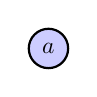
\begin{tikzpicture}[baseline=-0.5ex]
    \tikzset{tensor/.style = {minimum size = 0.5cm,shape = circle,thick,draw=black,inner sep = 0pt}, edge/.style = {thick,line width=.4mm},every loop/.style={}}
    \def\y{0}
    \def\x{0}
    \node[tensor,fill=blue!20!white] (a) at (\x,\y){\scalebox{0.85}{$a$}};
    \end{tikzpicture}%
    \ \ \ $\in \RR$,\hspace{0.01cm}
    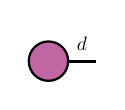
\begin{tikzpicture}[baseline=-0.5ex]
    \tikzset{tensor/.style = {minimum size = 0.5cm,shape = circle,thick,draw=black,inner sep = 0pt}, edge/.style = {thick,line width=.4mm},every loop/.style={}}
    \def\y{0}
    \def\x{0}
    \node[tensor,fill=blue!40!red!60!white] (a) at (\x,\y){\scalebox{0.85}{$\ab$}};
    \draw[edge] (\x+0.25,\y) -- (\x+0.6,\y)  node [midway,above] {\scalebox{0.7}{\dimcolor{$d$}}};
    \end{tikzpicture}
    $\in \RR^d$,\hspace{0.3cm}
    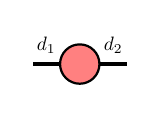
\begin{tikzpicture}[baseline=-0.5ex]
    \tikzset{tensor/.style = {minimum size = 0.5cm,shape = circle,thick,draw=black,inner sep = 0pt}, edge/.style = {thick,line width=.4mm},every loop/.style={}}
    \def\y{0}
    \def\x{0}
    \node[tensor,fill=red!50!white] (A) at (\x,\y){\scalebox{0.85}{$\Ab$}};
    \draw[edge] (\x+0.25,\y) -- (\x+0.6,\y)  node [midway,above] {\scalebox{0.7}{\dimcolor{$d_2$}}};
    \draw[edge] (\x-0.25,\y) -- (\x-0.6,\y)  node [midway,above] {\scalebox{0.7}{\dimcolor{$d_1$}}};
    \end{tikzpicture}
    \ \ \ $\in \RR^{d_1\times d_2}$,\hspace{0.3cm}
    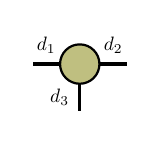
\begin{tikzpicture}[baseline=-0.5ex]
    \tikzset{tensor/.style = {minimum size = 0.5cm,shape = circle,thick,draw=black,inner sep = 0pt}, edge/.style = {thick,line width=.4mm},every loop/.style={}}
    \def\y{0}
    \def\x{0}
    \node[tensor,fill=green!50!red!50!white] (A) at (\x,\y){\scalebox{0.85}{$\At$}};
    \draw[edge] (\x+0.25,\y) -- (\x+0.6,\y)  node [midway,above] {\scalebox{0.7}{\dimcolor{$d_2$}}};
    \draw[edge] (\x-0.25,\y) -- (\x-0.6,\y)  node [midway,above] {\scalebox{0.7}{\dimcolor{$d_1$}}};
    \draw[edge] (\x,\y-0.25) -- (\x,\y-0.6)  node [midway,left] {\scalebox{0.7}{\dimcolor{$d_3$}}};
    \end{tikzpicture}
    \ \ \ $\in \RR^{d_1\times d_2\times d_3}$,\hspace{0.01cm}
    \begin{tikzpicture}[baseline=-0.5ex]
    \tikzset{tensor/.style = {minimum width = 1.8cm,minimum height = 0.4cm,shape = rounded rectangle,thick,draw=black,inner sep = 0pt}, edge/.style = {thick,line width=.4mm},every loop/.style={}}
    \def\x{0}
    \def\y{0}
    \draw[edge] (\x-0.2,\y-0.15) -- (\x-0.2,\y-0.6)node [midway,left=-0.05cm] {\scalebox{0.7}{\dimcolor{$d_2$}}};
    \draw[edge] (\x-0.6,\y-0.15) -- (\x-0.6,\y-0.6)node [midway,left=-0.05cm] {\scalebox{0.7}{\dimcolor{$d_1$}}};
    \draw[edge] (\x+0.2,\y-0.15) -- (\x+0.2,\y-0.6)node [midway,left=-0.05cm] {\scalebox{0.7}{\dimcolor{$d_3$}}};
    \draw[edge] (\x+0.6,\y-0.15) -- (\x+0.6,\y-0.6)node [midway,left=-0.05cm] {\scalebox{0.7}{\dimcolor{$d_4$}}};
    \node[tensor,fill=green!30!white] (Bt) at (\x,\y){$\Bt$};
    \end{tikzpicture}
    $\in \RR^{d_1\times d_2\times d_3\times d_4}$.
